\documentclass[a4paper, amsfonts, amssymb, amsmath, reprint, showkeys, nofootinbib, twoside, floatfix]{revtex4-2}
\usepackage[english]{babel}
\usepackage[utf8]{inputenc}
\usepackage{bm} % for bold math symbols
\usepackage[colorinlistoftodos, color=green!40, prependcaption]{todonotes}
\usepackage{booktabs}
\usepackage{comment}
\usetikzlibrary{positioning,chains}
\usepackage{tikz}
\usepackage{lipsum,adjustbox}
\usepackage{empheq} 
\usetikzlibrary{shapes,arrows,positioning}
\usetikzlibrary{fit, arrows.meta, shapes}
\usetikzlibrary{external}
\tikzexternalize % activate!
\newcommand{\subsubsubsection}[1]{\paragraph{#1}\mbox{}\\}
\setcounter{secnumdepth}{4}
\setcounter{tocdepth}{4}

\usepackage{amsthm}
\usepackage{mathtools}
\usepackage{listings}
\usepackage{physics}
\usepackage{xcolor}
\usepackage{graphicx}
\usepackage[left=23mm,right=13mm,top=35mm,columnsep=15pt]{geometry} 
\usepackage{adjustbox}
\usepackage{placeins}
\usepackage[T1]{fontenc}
\usepackage{lipsum}
\usepackage{csquotes}
\usepackage{algorithm}
\usepackage[noend]{algpseudocode}
\usepackage{svg}
\usepackage{url}
\usepackage{caption}
\usepackage{subcaption}
\usepackage{float}
\usepackage{enumitem}
\usepackage{siunitx}
\mathtoolsset{showonlyrefs=false} 
\usepackage{xcolor}
\usepackage{hyperref} % For hyperlinks in the PDF
%\setlength{\marginparwidth}{2.5cm}
\bibliographystyle{apsrev4-1}
%\bibliographystyle{apalike}
\usepackage{tikz}
\usetikzlibrary{quantikz}
% defines the color of hyperref objects
% Blending two colors:  blue!80!black  =  .8 blue and 0.2 black       % automagic cross-referencing
\hypersetup{ % this is just my personal choice, feel free to change things
    colorlinks,
    linkcolor={red!50!black},
    citecolor={blue!50!black},
    urlcolor={blue!80!black}}

\usepackage{listings}
\lstset{language=C, keywordstyle={\bfseries \color{blue}}}

\bibliographystyle{apsrev4-1}
\begin{document}
\include{amsmath}

\title{Learning chaotic dynamics with RNNs}
\email[]{https://github.com/Daniel-Haas-B/AdvancedMachineLearning}
\author{Daniel Haas}
\author{Keran Chen}
\affiliation{University of Oslo, Department of Physics}
\date{\today} % Leave empty to omit a date

\newcommand{\kc}[1]{\textcolor{green}{#1 $\mathcal{K}$}}
\newcommand{\dan}[1]{\textcolor{red}{#1 $\mathcal{D}$}}
\renewcommand{\eqref}[1]{Eq. (\ref{#1})}
\newcommand{\tabref}[1]{Tab. (\ref{#1})}
\newcommand{\figref}[1]{Fig. (\ref{#1})}


\begin{abstract}
% Motivation
 In this study, we delve into the challenge of predicting the dynamics of differential equations by leveraging the power of recurrent neural networks (RNNs). Our primary objective is to investigate how to employ different types of RNNs in dynamic systems while also assessing their performance in two distinct systems - one stable and one chaotic. We show that regular feed-forward neural networks (FFNNs) have difficulty in capturing the time dependency of the temporal data. We then show that RNNs can be used to get results from this time-series analysis, essentially by learning the dynamics of systems. For that, we train the network in different trajectories of Lorenz attractor simulations with different initial conditions.  We experiment with some hyperparameter tuning and show that using LSTM can yield better results than the standard RNN. We further motivate the introduction of physically informed loss functions to embed physical constraints to the neural network. Illustrating the difficulty of predicting chaotic dynamics, we also benchmark our methods by predicting stable spiral trajectories.
\end{abstract}

%\keywords{Ising Model, Feed-Forward Neural Network, Convolutional Neural Network}

\maketitle

\twocolumngrid
\section{Introduction}\label{introduction}

In 1963, the meteorologist and mathematician E. N. Lorenz unveiled an extraordinary system. By significantly reducing the complexity of a model for weather prediction, he came across a three-dimensional differential equation that demonstrated a phenomenon known as "deterministic chaos".

Upon employing certain constants, an extensive collection of solutions gravitate towards a set resembling the shape of a butterfly - hence dubbed the 'Lorenz Attractor'. This particular type of behavior is categorized as "chaos" \cite{zhang2022}.

The difficulty created by this set among many other sets of coupled differential equations is that they have no analytical solutions. Recently, advancements in machine learning and, more specifically, recurrent neural networks (RNNs), have provided us with a new way through which we can investigate this dynamic system.

In this report, we studied different ways to predict a time sequence with various complexities. Using time sequences generated by standard fourth-order Runge-Kutta (RK4) methods, we started by attempting to predict future steps using a standard Feed Forward Neural Network, then a simple RNN, and thereafter, LSTM RNNs with and without an added physics-informed loss function. We then compared their behaviors and explained why LSTM RNNs are best suited for studying this time series. Lastly, we also explored a less chaotic system, namely the stable spiral. The results proved to be very interesting.

The goal of this report is to provide our findings on how RNNs predict time series and chaotic systems and explain the difficulties and potential solutions, in an attempt to generate new insights.

In section \ref{methods}, we present an overview of RNNs and their basic ingredients, such as recurrent connections, hidden states, activation functions, and backpropagation through time. Subsequently, we present the physical model of Lorenz attractors to explain how we generated the data set via simulations and discuss how chaotic systems are hard to learn for an ML algorithm. We start section \ref{results}, by showing that a regular FFNN is unable to learn the proper dynamics of the chaotic motion for a satisfactory trajectory extrapolation.

Section \ref{discussion} analyses the obtained results, comparing the implemented methods and their ability to extract data from the model, noting possible future improvements.
In Section \ref{conclusion}, we conclude with a summary of what was learned from the several results and methods. 


  
\section{Methods}\label{methods}

\subsection{Data Set: a physics overview}\label{sec:data}

The field of dynamic systems encompasses a broad discipline, and a discussion of such can be approached both with a physics or a purely mathematical scope. A general but simple description is that it is the study of how a system evolves over time. For our purposes and investigations, we shall focus on the mathematical aspects of it, as we are interested in a dynamical system as a solution for a differential equation, which we face as a time-series evolution. Nonetheless, we will make use of physics tools in order to devise better-predicting algorithms.

A dynamical system can be categorized based on how it develops over time, but also how this behavior is affected by initial conditions and other rules. Two canonical examples of dynamical systems which exhibit completely different time evolution properties are the Lorenz attractor and a stable spiral.

\subsubsection{Stable Spiral}\label{sec:spiral}

The dynamics of a stable spiral evolve in such a way that the system's trajectory converges to a fixed point while spiraling inward. These oscillations around the fixed point are gradually dampened until the system reaches a steady state at a fixed point.
Suppose we have a two-dimensional system of coupled differential equations of the form

\begin{align}
    \frac{dx}{dt} &= ax + by \notag,\\
    \frac{dy}{dt} &= cx + dy.
    \label{eq:spiral}
\end{align}

The choice of $a,b,c,d \in \mathbb{R}$ completely determines the behavior of the solution, and for some of these values, albeit not all, the system is said to be a stable spiral. This condition is satisfied when the eigenvalues of the matrix formed by the coefficients are complex conjugates with a negative real part \cite{abell2022chapter6}. 

For illustration, \figref{fig:spiral} depicts the simulation of a stable spiral trajectory.

\begin{figure}[H]
\includegraphics[width= \linewidth]{figs/stable_spiral_a=0.2_b=1.0_c=1.0_d=0.2_plot.pdf}
    \caption{Trajectory of a simple stable spiral with coefficients $a = 0.2$, $b = -1.0$ , $c = 1.0$ , $d = 0.2$.}
    \label{fig:spiral}
\end{figure}


\subsubsection{Lorenz attractor}\label{sec:lorenz}

In contrast to the previous example, a Lorenz attractor presents some added complexity. Firstly, it is by definition a three-dimensional system, but more importantly, it exhibits what is called chaotic behavior \cite{hasselblatt2003first}. While there is no universal consensus on the definition of a chaotic system, all definitions agree chaotic systems are extremely sensitive to initial conditions. This means an arbitrary perturbation of such a set of conditions -or the current trajectory- will lead to vastly distinct asymptotic behavior.

The expression for the Lorenz attractor evolution consists of a set of three coupled nonlinear differential equations given by

\begin{align}
    \frac{dx}{dt} &= \sigma (y-x), \notag\\
    \frac{dy}{dt} &= x(\rho -z) - y, \notag\\
    \frac{dz}{dt} &= xy- \beta z.  
    \label{eq:lorenz}
\end{align}

For this problem, ${x,y,z}$ are the variables that determine the state of the system in the space while $\sigma, \rho$ and $\beta$ are, similarly to the constants $a,b,c,d$ of the stable spiral, parameters that influence largely how the system evolves. For illustration, \figref{fig:lorenz} depicts two particular Lorenz attractor trajectories.

\begin{figure}[H]
\includegraphics[width= \linewidth]{figs/lorenz.pdf}
    \caption{Simulation of two Lorenz attractor trajectories. While both are determined by \eqref{eq:lorenz}, they had two different initial conditions, hence the legend IC 1 and IC 2.}
    \label{fig:lorenz}
\end{figure}

\subsubsection{Generating the data}\label{sec:rk4}

Both of the above-mentioned systems are governed by differential equations, and as such, they can be solved numerically through some integration scheme such as forward-Euler or fourth-order Runge-Kutta. The latter was the algorithm of choice for the generated data sets.  

For our attractor, we will use the common choice of parameters $\sigma =10$, $\rho =28$, $\beta =8/3$. Although apparently arbitrary, this is a natural choice. Not only was it used by Lorenz himself \cite{lorenz1963deterministic}, but it generates complex and aesthetic trajectories that have been extensively investigated and benchmarked in the literature of numerical simulations. For the stable spiral, we used $a = 0.2$, $b = -1.0$, $c = 1.0$, $d = 0.2$ as it showed a good number of oscillations before reaching a steady state for our simulation time. 


\subsection{Feed-forward networks}
\begin{figure}[H]
\begin{center}
    

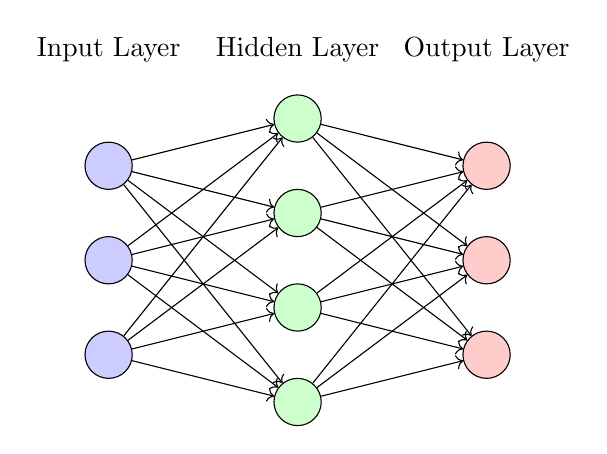
\begin{tikzpicture}[scale=1.2]
  % Input layer
  \foreach \i in {1,...,3}
    \node[circle, draw=black, fill=blue!20, minimum size=6mm] (input-\i) at (0,-\i) {};

  % Hidden layer
  \foreach \i in {1,...,4}
    \node[circle, draw=black, fill=green!20, minimum size=6mm] (hidden-\i) at (2,-\i+0.5) {};

  % Output layer
  \foreach \i in {1,...,3}
    \node[circle, draw=black, fill=red!20, minimum size=6mm] (output-\i) at (4,-\i) {};

  % Arrows
  \foreach \i in {1,...,3}
    \foreach \j in {1,...,4}
      \draw[->] (input-\i) -- (hidden-\j);

  \foreach \i in {1,...,4}
    \foreach \j in {1,...,3}
      \draw[->] (hidden-\i) -- (output-\j);

  % Labels
  \node[above] at (0,0) {Input Layer};
  \node[above] at (2,0) {Hidden Layer};
  \node[above] at (4,0) {Output Layer};
\end{tikzpicture}
\end{center}

    \caption{Basic schematic of a feed-forward neural network showing its layers and units.}
    \label{fig:ffn}
\end{figure}


In its general definition, a feed-forward neural network is a way to organize a set of function compositions in a sequential way. The algorithmic way of doing so is referred to as a network, given that it can be understood as being composed of individual but somehow connected units in a graph-like manner. 

The network is said to be of feed-forward type if information flows in one preferential direction in the network. This means each neuron receives inputs from the previous layer, and after multiplying it by a set of weights and adding some bias - and often composing it with some activation function - passes the result to neurons in the next layer. The way in which the units are organized in layers and how they are connected results in different architectures. 

The choice of the architecture of a network is often guided by the problem one aims at tackling, but most networks have some overlapping core structure in the form of input layers, hidden layers, output layers, and activation functions, as can be seen in \figref{fig:ffn}. The network's weights and biases are then iteratively updated via a gradient scheme that tries to converge to a global minimum of a cost-function. This cost function is a measurement of well the model performs, be it in regression, or classification problems.


\begin{align}
&            && \mathbf{h}_0 = \mathbf{x} \notag\\
&            && 
                \negthickspace% for compensation of rcases misalignment
                \begin{rcases}  
                \mathbf{a}_i= W_i * \mathbf{h}_{i-1} + \mathbf{b}_i \notag\\
                \mathbf{h}_i    = \sigma_i(\mathbf{a}_i) 
                    \end{rcases}&  i \in \{1, ..., L-1\}, \\
&            &&\mathbf{\hat{y}} = \sigma_L(W_y *\mathbf{h}_{L-1} + \mathbf{b}_y) 
\label{eq:FFN}
\end{align}

where $W_i$ and $b_i$ are respectively the weight matrix and bias vector of the i-th layer, $h_i$ represents the output of the i-th hidden layer and we are defining the 0-th hidden layer as the input of the network, $\mathbf{x}$. Similarly, $\sigma_i$ represents the activation function of each hidden layer and $L$ is the output layer. 

There are limitation of FFNNs, one of which being that FFNNs are not designed to handle sequential data (data for which the order matters) effectively because they lack the capabilities of storing information about previous inputs; each input is being treated independently. This is a limitation when dealing with sequential data where past information can be vital to correctly process current and future inputs.

\subsection{Recurrent networks}

In contrast to FFNs, recurrent networks introduce feedback connections, meaning the information is allowed to be carried to subsequent nodes across different time steps. These cyclic or feedback connections have the objective of providing the network with some kind of memory, making RNNs particularly suited for time-series data, natural language processing, speech recognition, and several other problems for which the order of the data is crucial. 

RNN architectures vary greatly in how they manage information flow and memory in the network. Different architectures often aim at improving some sub-optimal characteristics of the network. The simplest form of recurrent network, commonly called simple or vanilla RNN, for example, is known to suffer from the problem of vanishing gradients.
This problem arises due to the nature of backpropagation in time. Gradients of the cost/loss function may get exponentially small (or large) if there are many layers in the network, which is the case of RNN when the sequence gets long. Consequently, the convergence to correctly predicted values in the training process happens very slowly. This is particularly the case when using activation functions like the Sigmoid or hyperbolic tangent, (whose outputs are between 0 and 1 for Sigmoid, and -1 and 1 for $\tanh$), with equally small gradients by design ($<1$).

To address that, one natural alternative is to use the Long Short-Term Memory (LSTM) variation. While LSTMs are generally used, they also present the downside of being inefficient for large-scale models. For such problems, Gated recurrent units (GRUs) can be employed as they have a simpler architecture, thus being computationally faster. We will hereafter focus simply on the Vanilla and LSTM variants for their simplicity and popularity.

\subsubsection{Vanilla RNN}

The expression for the simplest Recurrent network resembles that of a regular feed-forward neural network of \eqref{eq:FFN}, but now with the concept of temporal dependencies as shown in the equations for the forward pass, \eqref{eq:rnn_forward},

\begin{align}
    \mathbf{a}^{(t)} & = U * \mathbf{x}^{(t)} + W * \mathbf{h}^{(t-1)} + \mathbf{b}, \notag \\
    \mathbf{h}^{(t)} &= \sigma_h(\mathbf{a}^{(t)}), \notag\\
    \mathbf{o}^{(t)} &= V * \mathbf{h}^{(t)} + \mathbf{c}, \notag\\
    \mathbf{\hat{y}}^{(t)} &= \sigma_y(\mathbf{o}^{(t)}).
    \label{eq:rnn_forward}
\end{align}

\onecolumngrid
\begin{center}

\begin{figure}
    \begin{adjustbox}{width=0.8\textwidth}
    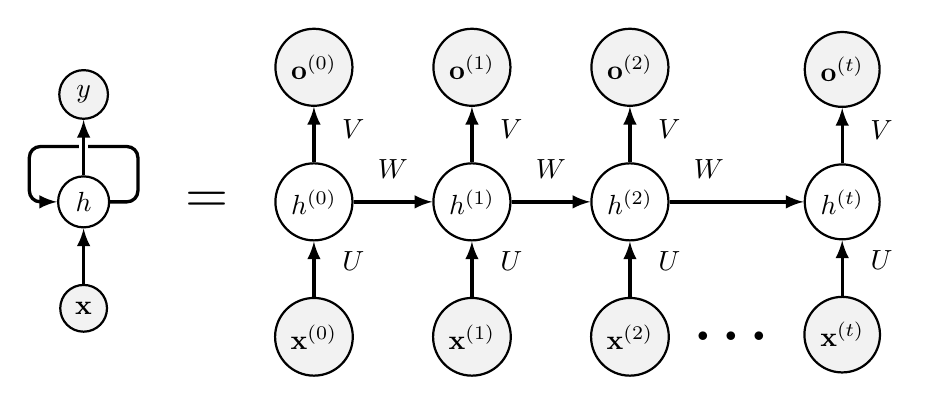
\begin{tikzpicture}[item/.style={circle,draw,thick,align=center},
itemc/.style={item,on chain,join}]
 \begin{scope}[start chain=going right,nodes=itemc,every
 join/.style={-latex,very thick},local bounding box=chain]
 \path node (A0) {$h^{(0)}$} node (A1) {$h^{(1)}$} node (A2) {$h^{(2)}$} node[xshift=2em] (At)
 {$h^{(t)}$};
 \end{scope}
 \node[left=1em of chain,scale=2] (eq) {$=$};
 \node[left=2em of eq,item] (AL) {$h$};
 \path (AL.west) ++ (-1em,2em) coordinate (aux);
 \draw[very thick,-latex,rounded corners] (AL.east) -| ++ (1em,2em) -- (aux) 
 |- (AL.west);
 \foreach \X in {0,1,2,t} 
     {\draw[very thick,-latex] (A\X.north) -- ++ (0,2em)
     node[above,item,fill=gray!10] (h\X) {$\mathbf{o}^{(\X)}$};
     %\ifthenelse{\X!=t;}{ \path (A\X.east) -- ++ (1,1em) node[midway, above] {$W$};};
     \draw[very thick,latex-] (A\X.south) -- ++ (0,-2em)
     node[below,item,fill=gray!10] (x\X) {$\mathbf{x}^{(\X)}$};}
 \draw[white,line width=0.8ex] (AL.north) -- ++ (0,1.9em);
 \draw[very thick,-latex] (AL.north) -- ++ (0,2em)
 node[above,item,fill=gray!10] {$y$};

 \draw[very thick,latex-] (AL.south) -- ++ (0,-2em)
 node[below,item,fill=gray!10] {$\mathbf{x}$};
 \path (x2) -- (xt) node[midway,scale=2,font=\bfseries] {\dots};

\foreach \X in {0,1,2} 
    \path (A\X.east) -- ++ (1,1em) node[midway, above] {$W$};
\foreach \X in {0,1,2, t} 
    \path (A\X.north) -- ++ (1,1em) node[midway, above] {$V$};
\foreach \X in {0,1,2,t} 
    \path (A\X.south) -- ++ (1,0em) node[midway, below] {$U$};
\end{tikzpicture}
\end{adjustbox}
    \caption{Folded versus unfolded representation of a Vanilla RNN}
    \label{fig:rnn}
\end{figure}
\end{center}

\twocolumngrid

Equation \eqref{eq:rnn_forward},  can be better understood from the schematics of \figref{fig:rnn}. Here, the superscripts denote the temporal dependency of each pass. As usual, $\mathbf{h}$ represents the output of the hidden layer, after its activation $\sigma_h$, while $\mathbf{y}$ and $\sigma_y$ have the analogous role for the output layer. Similarly to a regular FFN, $\mathbf{b} $ and $\mathbf{c}$ represent the bias of the hidden layers and the output layers respectively. Notice however that we have weight matrices that modulate two inputs to a fixed hidden layer, $U$ and $W$. Indeed, hidden layers now receive a temporal input of the data $\mathbf{x}^{(t)}$ but also from the output of the same hidden layer in a previous temporal step, $\mathbf{h}^{(t-1)}$. Finally, the output layer's input is also modulated by weights $V$.

For this breakdown of equation \eqref{eq:rnn_forward} it is important to note that we are not specifying which layer of the network we are propagating, to avoid carrying indices. As can be seen from \figref{fig:rnn}, RNNs are often depicted in both a folded and an unfolded visualization, but it is important to note that a unit $h^{(t)}$ can be composed of many layers.

The learning procedure for RNNs also follows the same idea as that of regular FFNs: we need to optimize weights and bias so that the loss function $\mathcal{L}$ which assesses how well the model performs, gets minimized. To construct $\mathcal{L}$, it is paramount it takes into account all the temporal outputs, $\mathbf{y}^{(t)}$, and sum over their respective losses,

\begin{align}
    \mathcal{L}= \sum_t L^{(t)}.
    \label{eq:loss_rnn}
\end{align}

The choice of the individual losses $L^{(t)}$ is heavily dependent on the problem at hand, and shall be discussed in the following section \ref{sec:loss_funct}. This temporal dependency of the loss means the usual back-propagation process to evaluate the gradient of the parameters and update them depends on previous time steps due to the chain rule. For that reason, it is called back-propagation through time (BPTT), but the idea behind it is the same as for regular back-propagation: derive the loss function with respect to the parameters.

\subsubsection{Backpropagation through time}

The subsequent derivation follows closely the explanations of \cite{Goodfellow}, however, we shall not assume any loss function for now. To derive the expression of the gradients of $\mathcal{L}$ for the RNN, we need to start recursively from the nodes closer to the output layer in the temporal unrolling scheme - such as $\mathbf{o}$ and $\mathbf{h}$ at final time $t = \tau$,

\begin{align}
    (\nabla_{ \mathbf{o}^{(t)}} \mathcal{L})_{i} &= \frac{\partial \mathcal{L}}{\partial L^{(t)}}\frac{\partial L^{(t)}}{\partial o_{i}^{(t)}}, \notag\\
    \nabla_{\mathbf{h}^{(\tau)}} \mathcal{L} &= \mathbf{V}^\mathsf{T}\nabla_{ \mathbf{o}^{(\tau)}} \mathcal{L}.
    \label{eq:rnn_gradients1}
\end{align}

For the following hidden nodes, we have to iterate through time, so by the chain rule, 

\begin{align}
    \nabla_{\mathbf{h}^{(t)}} \mathcal{L} &= \left(\frac{\partial\mathbf{h}^{(t+1)}}{\partial\mathbf{h}^{(t)}}\right)^\mathsf{T}\nabla_{\mathbf{h}^{(t+1)}}\mathcal{L} + \left(\frac{\partial\mathbf{o}^{(t)}}{\partial\mathbf{h}^{(t)}}\right)^\mathsf{T}\nabla_{ \mathbf{o}^{(t)}} \mathcal{L}.
    \label{eq:rnn_gradients2}
\end{align}

Similarly, the gradients of $\mathcal{L}$ with respect to the weights and biases follow,

\begin{align}
    \nabla_{\mathbf{c}} \mathcal{L} &=\sum_{t}\left(\frac{\partial \mathbf{o}^{(t)}}{\partial \mathbf{c}}\right)^\mathsf{T} \nabla_{\mathbf{o}^{(t)}} \mathcal{L} \notag\\
    \nabla_{\mathbf{b}} \mathcal{L} &=\sum_{t}\left(\frac{\partial \mathbf{h}^{(t)}}{\partial \mathbf{b}}\right)^\mathsf{T}        \nabla_{\mathbf{h}^{(t)}} \mathcal{L} \notag\\
    \nabla_{\mathbf{V}} \mathcal{L} &=\sum_{t}\sum_{i}\left(\frac{\partial \mathcal{L}}{\partial o_i^{(t)} }\right)\nabla_{\mathbf{V}^{(t)}}o_i^{(t)} \notag\\
    \nabla_{\mathbf{W}} \mathcal{L} &=\sum_{t}\sum_{i}\left(\frac{\partial \mathcal{L}}{\partial h_i^{(t)}}\right)\nabla_{\mathbf{w}^{(t)}} h_i^{(t)} \notag\\
    \nabla_{\mathbf{U}} \mathcal{L} &=\sum_{t}\sum_{i}\left(\frac{\partial \mathcal{L}}{\partial h_i^{(t)}}\right)\nabla_{\mathbf{U}^{(t)}}h_i^{(t)}.
    \label{eq:rnn_gradients3}
\end{align}


The pseudo-code in \ref{algo:bptt} illustrates algorithmically how information and the gradients flow in a vanilla RNN based on the previous equations of \eqref{eq:rnn_gradients1}, \eqref{eq:rnn_gradients2} and \eqref{eq:rnn_gradients3}. Note that it already assumes the bias and weights to be initialized - for such, it is usual to use normal random distribution $\mathcal{N}(0, \sigma)$, where $\sigma$ is small to prevent exploding gradients.

\begin{figure}
    \begin{algorithm}[H]
    \caption{ Single Vanilla RNN epoch}
    \label{algo:bptt}
        \begin{algorithmic}
            \State $\boldsymbol{\delta_h},\boldsymbol{\delta_W},\boldsymbol{\delta_V},\boldsymbol{\delta_b},\boldsymbol{\delta_c}  = \mathbf{0}$ \Comment{Initialize gradient accumulation states}
            \For {each time step $t$ in the sequence}
                \State $\mathbf{o}^{(t)}$, $\mathbf{h}^{(t)}$ $\leftarrow$ \textbf{Forward pass}
            \EndFor
            \State $\mathcal{L}\leftarrow$ \textbf{Compute loss} 
            \State \textbf{Compute gradient of output layer:}
            \State $(\nabla_{ \mathbf{o}^{(t)}} \mathcal{L})_{i} $ \Comment{Based on specific loss}
            \State \textbf{Compute gradient of hidden layer at $t = \tau$:}
            \State $\boldsymbol{\delta_h} \leftarrow \nabla_{\mathbf{h}^{(\tau)}} \mathcal{L} $ 
            \State \textbf{Backpropagate through time:}
            \For {each time step $t = \tau - 1$ to $t=1$}
                \State \textbf{Compute and update hidden state gradient:}
                \State $\boldsymbol{\delta_h} = \left(\frac{\partial\mathbf{h}^{(t+1)}}{\partial\mathbf{h}^{(t)}}\right)^\mathsf{T}\boldsymbol{\delta_h} + \left(\frac{\partial\mathbf{o}^{(t)}}{\partial\mathbf{h}^{(t)}}\right)^\mathsf{T}\nabla_{ \mathbf{o}^{(t)}} \mathcal{L}$ 

                \State \textbf{Acumulate parameter gradients:}
                \State $\boldsymbol{\delta_c} += \left(\frac{\partial \mathbf{o}^{(t)}}{\partial\mathbf{c}}\right)^\mathsf{T}\nabla_{\mathbf{o}^{(t)}} \mathcal{L}$
                \State $\boldsymbol{\delta_b} += \left(\frac{\partial \mathbf{h}^{(t)}}{\partial\mathbf{b}}\right)^\mathsf{T}\nabla_{\mathbf{h}^{(t)}} \mathcal{L}$
                \State $\boldsymbol{\delta_V} +=\sum_{i} \left(\frac{\partial \mathcal{L}}{\partial o_{i}^{(t)}}\right)\nabla_{\mathbf{V}^{(t)}}o^{(t)}_{i}$
                \State $\boldsymbol{\delta_W} +=\sum_{i} \left( {\delta_{\mathbf{h}}}\right)_i\nabla_{\mathbf{W}^{(t)}}h^{(t)}_{i}$
                \State $\boldsymbol{\delta_U} +=\sum_{i} \left( {\delta_{\mathbf{h}}}\right)_i\nabla_{\mathbf{U}^{(t)}}h^{(t)}_{i}$
            \EndFor
            \State \textbf{Weight and bias update:}
            \State $\enspace \{W, U, V, \mathbf{b}, \mathbf{c} \}-= \alpha \cdot  \{\boldsymbol{\delta_W} , \boldsymbol{\delta_U} , \boldsymbol{\delta_V} , \boldsymbol{\delta_b} ,\boldsymbol{\delta_c} \}$
        \end{algorithmic}
    \end{algorithm}
    \caption*{Pseudo code for the forward and backward propagations of a simple RNN. Equations for the gradient expressions follow \eqref{eq:rnn_gradients1}, \eqref{eq:rnn_gradients2}, \eqref{eq:rnn_gradients3}}
\end{figure}


\subsubsection{LSTM}
The Long Short Term Memory RNN is a type of RNN designed to avoid the vanishing or exploding gradient caused easily by the Vanilla RNN, which makes it difficult to learn long-range dependencies in a sequence.  Given the recurrent relation in equation \eqref{eq:rnn_gradients2}, the long-term gradient can end up having many factors of $\partial \mathbf{h}^{(t+1)}/\partial\mathbf{h}^{(t)}$, which may be close to zero or excessively large, leading to vanishing or exploding gradients respectively. In 1997, in order to address the aforementioned problem, Hochreiter and Schmidhuber introduced LSTM which truncates the gradient where it does not incur significant detriment to performance \cite{Hochreiter97}.

The LSTM is a unit cell that is made of three gates: the input gate, the forget gate, and the output gate. It also introduces a cell state $c$, which can be thought of as the long-term memory, and a hidden state $h$ which can be thought of as the short-term memory. As illustrated in Figure~\ref{fig:lstm}. \\
The first stage is called the forget gate, where we combine the input at (say, time $t$), and the hidden cell state input at $t-1$, passing it through the Sigmoid activation function and then performing an element-wise multiplication, denoted by $\otimes$.
It follows 
\[\mathbf{f}^{(t)} = \sigma(W_f\mathbf{x}^{(t)} + U_f\mathbf{h}^{(t-1)} + \mathbf{b}_f) \]
where $W$ and $U$ are the weights respectively.
This is called the forget gate since the Sigmoid activation function's outputs are very close to $0$ if the argument for the function is very negative, and $1$ if the argument is very positive. Hence we can control the amount of information we want to take from the long-term memory.\\

The next stage is the input gate, which consists of both a Sigmoid function ($\sigma_i$), which decide what percentage of the input will be stored in the long-term memory, and the $\tanh_i$ function, which decide what is the full memory that can be stored in the long term memory. When these results are calculated and multiplied together, it is added to the cell state or stored in the long-term memory, denoted as $\oplus$. \\
It follows
\[\mathbf{i}^{(t)} = \sigma_g(W_i\mathbf{x}^{(t)} + U_i\mathbf{h}^{(t-1)} + \mathbf{b}_i),\]
\[\mathbf{\tilde{c}}^{(t)} = \tanh(W_c\mathbf{x}^{(t)} + U_c\mathbf{h}^{(t-1)} + \mathbf{b}_c),\] again the $W$ and $U$ are the weights.

The forget gate and the input gate together also update the cell state with the following equation, 
\[\mathbf{c}^{(t)} = \mathbf{f}^{(t)} \otimes \mathbf{c}^{(t-1)} + \mathbf{i}^{(t)} \otimes \mathbf{\tilde{c}}^{(t)},\] where $f^{(t)}$ and $i^{(t)}$ are the outputs of the forget gate and the input gate, respectively.

The final stage of the LSTM is the output gate, and  its purpose is to update the short-term memory.  To achieve this, we take the newly generated long-term memory and process it through a hyperbolic tangent ($\tanh$) function creating a potential new short-term memory. We then multiply this potential memory by the output of the Sigmoid function ($\sigma_o$). This multiplication generates the final output as well as the input for the next hidden cell ($h^{\langle t \rangle}$) within the LSTM cell.


It follows,
\[\begin{aligned}
\mathbf{o}^{(t)} &= \sigma_g(W_o\mathbf{x}^{(t)} + U_o\mathbf{h}^{(t-1)} + \mathbf{b}_o), \\
\mathbf{h}^{(t)} &= \mathbf{o}^{(t)} \otimes \sigma_h(\mathbf{c}^{(t)}). \\
\end{aligned}\]
where $\mathbf{W_o,U_o}$ are the weights of the output gate and $\mathbf{b_o}$ is the bias of the output gate.

\begin{figure}
    \centering
    
\newcommand{\empt}[2]{$#1^{\langle #2 \rangle}$}

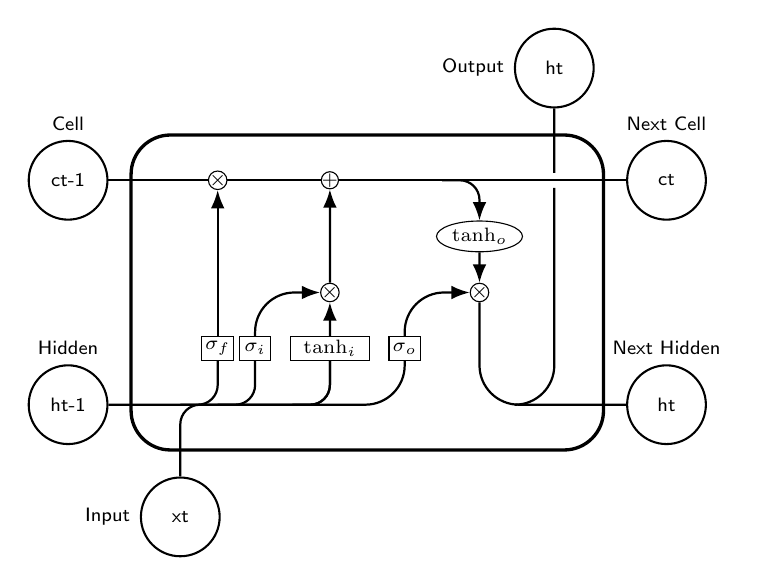
\begin{tikzpicture}[scale=0.95,
    % GLOBAL CFG
    font=\sf \scriptsize,
    >=LaTeX,
    % Styles
    cell/.style={% For the main box
        rectangle, 
        rounded corners=5mm, 
        draw,
        very thick,
        },
    operator/.style={%For operators like +  and  x
        circle,
        draw,
        inner sep=-0.5pt,
        minimum height =.2cm,
        },
    function/.style={%For functions
        ellipse,
        draw,
        inner sep=1pt
        },
    ct/.style={% For external inputs and outputs
        circle,
        draw,
        line width = .75pt,
        minimum width=1cm,
        inner sep=1pt,
        },
    gt/.style={% For internal inputs
        rectangle,
        draw,
        minimum width=4mm,
        minimum height=3mm,
        inner sep=1pt
        },
    mylabel/.style={% something new that I have learned
        font=\scriptsize\sffamily
        },
    ArrowC1/.style={% Arrows with rounded corners
        rounded corners=.25cm,
        thick,
        },
    ArrowC2/.style={% Arrows with big rounded corners
        rounded corners=.5cm,
        thick,
        },
    ]

%Start drawing the thing...    
    % Draw the cell: 
    \node [cell, minimum height =4cm, minimum width=6cm] at (0,0){} ;

    % Draw inputs named ibox#
    \node [gt] (ibox1) at (-2,-0.75) {$\sigma_f$};
    \node [gt] (ibox2) at (-1.5,-0.75) {$\sigma_i$};
    \node [gt, minimum width=1cm] (ibox3) at (-0.5,-0.75) {$\tanh_i$};
    \node [gt] (ibox4) at (0.5,-0.75) {$\sigma_o$};

   % Draw opérators   named mux# , add# and func#
    \node [operator] (mux1) at (-2,1.5) {$\times$};
    \node [operator] (add1) at (-0.5,1.5) {+};
    \node [operator] (mux2) at (-0.5,0) {$\times$};
    \node [operator] (mux3) at (1.5,0) {$\times$};
    \node [function] (func1) at (1.5,0.75) {$\tanh_o$};

    % Draw External inputs? named as basis c,h,x
    \node[ct, label={[mylabel]Cell}] (c) at (-4,1.5) {\empt{c}{t-1}};
    \node[ct, label={[mylabel]Hidden}] (h) at (-4,-1.5) {\empt{h}{t-1}};
    \node[ct, label={[mylabel]left:Input}] (x) at (-2.5,-3) {\empt{x}{t}};

    % Draw External outputs? named as basis c2,h2,x2
    \node[ct, label={[mylabel]Next Cell}] (c2) at (4,1.5) {\empt{c}{t}};
    \node[ct, label={[mylabel]Next Hidden}] (h2) at (4,-1.5) {\empt{h}{t}};
    \node[ct, label={[mylabel]left:Output}] (x2) at (2.5,3) {\empt{h}{t}};

% Start connecting all.
    %Intersections and displacements are used. 
    % Drawing arrows    
    \draw [ArrowC1] (c) -- (mux1) -- (add1) -- (c2);

    % Inputs
    \draw [ArrowC2] (h) -| (ibox4);
    \draw [ArrowC1] (h -| ibox1)++(-0.5,0) -| (ibox1); 
    \draw [ArrowC1] (h -| ibox2)++(-0.5,0) -| (ibox2);
    \draw [ArrowC1] (h -| ibox3)++(-0.5,0) -| (ibox3);
    \draw [ArrowC1] (x) -- (x |- h)-| (ibox3);

    % Internal
    \draw [->, ArrowC2] (ibox1) -- (mux1);
    \draw [->, ArrowC2] (ibox2) |- (mux2);
    \draw [->, ArrowC2] (ibox3) -- (mux2);
    \draw [->, ArrowC2] (ibox4) |- (mux3);
    \draw [->, ArrowC2] (mux2) -- (add1);
    \draw [->, ArrowC1] (add1 -| func1)++(-0.5,0) -| (func1);
    \draw [->, ArrowC2] (func1) -- (mux3);

    %Outputs
    \draw [-, ArrowC2] (mux3) |- (h2);
    \draw (c2 -| x2) ++(0,-0.1) coordinate (i1);
    \draw [-, ArrowC2] (h2 -| x2)++(-0.5,0) -| (i1);
    \draw [-, ArrowC2] (i1)++(0,0.2) -- (x2);

\end{tikzpicture}

\caption{LSTM illustration \footnote{source: https://tex.stackexchange.com/questions/432312/how-do-i-draw-an-lstm-cell-in-tikz}}
    \label{fig:lstm}
\end{figure}


\subsubsection{Training and testing trajectories}

Training and testing procedures in recurrent neural networks follow what is usual for regular FNNs, but some special consideration needs to be taken into account due to the sequential character of the data. Training and testing batches must not be randomly shuffled for it would clearly decorrelate the time-series points and leak future information into present or past points of the model. 

Additionally, the training algorithm in Algorithm (\ref{algo:bptt}) can become computationally costly, especially if the losses are evaluated for all previous time steps. While other architectures such as that of GRUs can be used to mitigate that, it is also possible to introduce another hyperparameter responsible for controlling how much of the network will be unfolded in the training process, adjusting how much the network will remember from previous points in time. We called this parameter the \emph{look-back}. Similarly, the number of steps the network predicts in the future per iteration greatly influences the assessment of the loss function. we called this parameter the \emph{look-ahead}.

The training and testing batches were separated into whole trajectories. This means that instead of training and testing on different fractions of the same trajectory, all trajectories that were tested had completely new initial conditions. In this sense, from a total of 10 initial conditions (independent trajectories), 9 were used for training and 1 for testing. Each trajectory consisted of 800 points in each space coordinate.

\subsection{On the choice of the loss function}  \label{sec:loss_funct}

Our problem is essentially a time-series forecasting problem, so, we are free to choose the loss function amongst the big collection of regression losses. Using the mean-squared error of the predicted versus factual trajectories of the dynamic systems is a natural choice for it is a way to measure their discrepancy in space, and it punished outliers strongly for its quadratic form. Furthermore, it is a convex function, so given sufficient time and appropriate learning rates, it is guaranteed to converge to global minima irrespective of the weight's random initialization. For completeness' sake, the expression for this loss function can be written 

\begin{align}
    \mathcal{L}_{MSE} = \frac{1}{N}\sum_{i}^N (y(\mathbf{x}_i) - \hat{y}(\mathbf{x}_i, \mathbf{\theta}))^2
    \label{eq:mse_loss}
\end{align}

where we are denoting $\mathbf{\theta}$ as the set of all parameters of the network, and $\mathbf{x}_i$ is our input. 

\subsubsection{The "naivety" of data-driven losses}

Simply using a loss function that is based on the observational and predicted data, such as the one in equation \eqref{eq:mse_loss} is commonly referred to as a purely data-driven approach. While this is a well-established way of assessing regressions, it does not make use of other intuitions we might have over the problem we are trying to solve. At the same time, it is a well-established fact that neural network models are data-greedy - they need large amounts of data to be able to generalize predictions outside the training set. One way to try to mitigate this is by using  physics-informed neural networks (PINNs) when possible.

Trying to improve the performance of our model beyond training sets, PINNs then add physics-informed penalties to the loss function. In essence, this means that we add a worse evaluation score to predictions that do not respect physical laws we think our real data should obey. This procedure often has the advantage of trimming the parameter space without adding bias to the model if the constraints imposed are correct, but the choice of the physical laws can be a delicate one. 


\subsubsection{Adding physics to the loss function}

A general way of expressing this added penalty to the loss function is shown in \eqref{eq:custom_loss} below,

\begin{align}
    \mathcal{L} = w_{MSE}\mathcal{L}_{MSE} + w_{PI}\mathcal{L}_{PI}.
    \label{eq:custom_loss}
\end{align}

Here, the weights $w_{MSE}$ and $w_{PI}$ explicitly mediate how much influence the specific parts of the total loss function should contribute. In our experimentations with the additional physics penalty, we limited results to only have $w_{MSE} = 1.0$ and $w_{PI}= 0.5$.

For one, it is important to note that this procedure is not a universal strategy to predict time-series data. In a general sense, the system need not obey the laws of physics. For instance, the Lorenz attractor, given its attractor behavior, does not conserve momentum.

While we are working with RNNs, the general schematics behind PINNs is illustrated in \figref{fig:PINNs} using a feed-forward net. The standard approach to construct $\mathcal{L}_{PI}$ is to ensure the outputs of the network satisfies the differential equations at hand. The outputs of the NN are often differentiated via an automatic differentiation software such as JAX \cite{jax2018github}. In our case, a natural approach would be

\begin{align}
    \mathcal{L}_{PI} &=     \frac{d \hat{x}}{dt} - \sigma (\hat{y}-\hat{x}) \notag\\
    & + \frac{d\hat{y}}{dt} - \hat{x}(\rho -\hat{z}) - \hat{y} \notag\\
    & +\frac{d\hat{z}}{dt} - \hat{x}\hat{y}- \beta \hat{z},
\end{align}

where we denoted with hats the neural network outputs. As long as the dynamics of the predictions respect the differential equations, this loss will be minimized. However, since we are working with recurrent neural networks that output one predicted time-step at a time during the training process, taking the derivative in time would not be straightforward. For this reason, we approach the problem of adding physics to the RNN in a similar but subtly different way. 

\begin{figure}[H]
\begin{center}
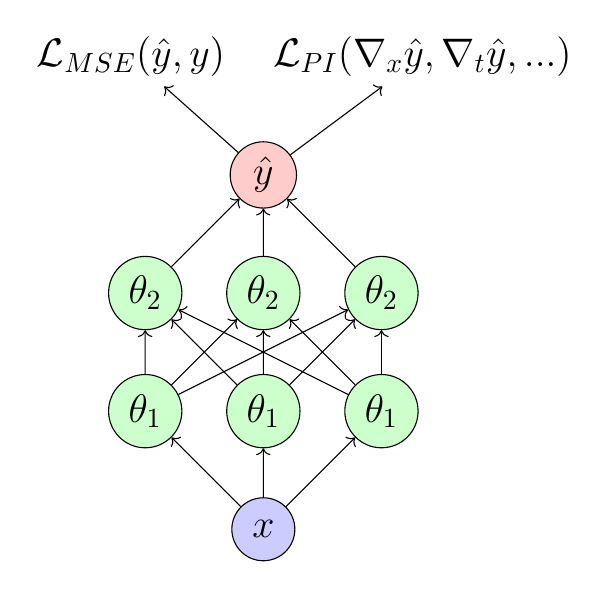
\begin{tikzpicture}[scale=1.5]
  % Input layer
  \foreach \i in {1}
    \node[circle, draw=black, fill=blue!20, minimum size=8mm] (input-\i) at (-\i, 0) {\Large $x$};

  % Hidden layer
  \foreach \i in {1,...,3}
    \node[circle, draw=black, fill=green!20, minimum size=8mm] (hidden1-\i) at (-\i+1, 1) {\Large
 $\theta_{1} $};

  \foreach \i in {1,...,3}
    \node[circle, draw=black, fill=green!20, minimum size=8mm] (hidden2-\i) at (-\i+1, 2) {\Large
 $\theta_{2} $};

  % Output layer
  \foreach \i in {1}
    \node[circle, draw=black, fill=red!20, minimum size=8mm] (output-\i) at (-\i , 3 ) {\Large $\hat{y}$};

 % eq layer
  \foreach \i in {1}
    \node[right] (equation1-\i) at (-\i, 4) {\Large
 $\mathcal{L}_{PI}(\nabla_x \hat{y},  \nabla_t \hat{y}, ...)$};

   \foreach \i in {1}
    \node[right] (equation2-\i) at (-\i - 2, 4) {\Large
 $\mathcal{L}_{MSE}(\hat{y}, y)$};


  % Arrows
  \foreach \i in {1}
    \foreach \j in {1,...,3}
      \draw[->] (input-\i) -- (hidden1-\j);
    
  \foreach \i in {1,...,3}
    \foreach \j in {1,...,3}
      \draw[->] (hidden1-\i) -- (hidden2-\j);

  \foreach \i in {1,...,3}
    \foreach \j in {1}
      \draw[->] (hidden2-\i) -- (output-\j);

    \draw[->](output-1) -- (equation1-1);
    \draw[->](output-1) -- (equation2-1);

\end{tikzpicture}
\end{center}
\caption{Sketch of the concurrent assessment of both physics-informed and data-driven losses.}
\label{fig:PINNs}
\end{figure}


As mentioned, the Lorenz attractor does not conserve momentum. Therefore, we cannot simply add a penalty term for when the subsequent temporal values of the right-hand side (RHS) of the differential equations (DE) (\ref{eq:lorenz}) differ from the initial one. To still enforce learning of the differential equation we instead construct the RHS of the DE from the positions predictions during training. We then compare those values with the same RHS of the DEs given the true trajectories. More specifically, the added physics loss was given by

\begin{align}
    \mathcal{L}_{PI} &=    MSE(\sigma (y-x), \sigma (\hat{y}-\hat{x})) \notag \\
    & + MSE(x(\rho -z) - y , \hat{x}(\rho -\hat{z}) - \hat{y}) \notag \\
    & +MSE(xy- \beta z , \hat{x}\hat{y}- \beta \hat{z})
\end{align}

The physics-informed term in the custom loss function represents the difference between the predicted derivatives of the Lorenz system and the true derivatives, as defined by the Lorenz equations. In other words, it measures how well the predicted trajectories of the system obey the physical laws that govern the Lorenz system.

By incorporating this physics-informed term into the loss function, the LSTM is encouraged to generate predictions that are not only accurate but also physically meaningful. This is important because the Lorenz system is a highly nonlinear and chaotic system, and therefore making predictions, especially long ones, is a hard task.
\section{Results}\label{results}


\subsubsection{Regular FFNN} 

We start by investigating how well a regular feed-forward neural network is able to predict the trajectories of the Lorenz attractor. By training on 9 trajectories with different initial conditions and testing on one, we generate the graph of \figref{fig:ffn_lorenz3d}. This figure was obtained with a three-layer network, where the number of nodes in each was, respectively, 64, 32, and 3.


\begin{figure}[H]
\includegraphics[width= \linewidth]{figs/lorenz_ffn_3d.pdf}
    \caption{Predicted versus test trajectories for the FFNN on the Lorenz attractor.}
    \label{fig:ffn_lorenz3d}
\end{figure}

For the loss function in this implementation, we used the mean absolute error and an Adam optimizer with a learning rate of $10^{-3}$. The training process was of 200 epochs, and \figref{fig:history_ffn} shows how the validation loss evolves in comparison to the training set loss throughout the training. The metric used for training this network was the mean absolute error, but the $y$-axis is shown as the mean absolute error (MAE) divided by the average of the trajectory's coordinates.

\begin{figure}[H]
\includegraphics[width= \linewidth]{figs/history_ffn.pdf}
    \caption{Training history of the FFNN for the prediction of Lorenz attractor. $y$-axis is shown as the MAE divided by the average of the trajectory's coordinates.}
    \label{fig:history_ffn}
\end{figure}

\figref{fig:ffn_lorenz} decomposes the coordinates of the trajectory used for testing the predictions, giving a more clear visualization than the 3D representation. 

\begin{figure}[H]
\includegraphics[width= \linewidth]{figs/lorenz_ffn.pdf}
    \caption{Testing versus predicted trajectories decomposed by coordinates for the FFNN.}
    \label{fig:ffn_lorenz}
\end{figure}


\subsubsection{Building an RNN with TensorFlow}\label{subsubsection:RNN_TF}

Aiming at investigating the RNN variants at their best, we start a series of basic hyperparameters gridsearch. More specifically, we begin investigating how the accuracy of the stable spiral predictions changes for different hyperparameters. In that sense, \figref{fig:hyperparams_vanilla_spiral} shows the gridsearch of the number of epochs of training versus the length of the sequence the network is retroactively trained on for each step - the \emph{look-back} parameter.


\begin{figure}
    \centering
\includegraphics[width= \linewidth]{figs/sprial_gridsearch_lenght_epochs_vanilla.pdf}
    \caption{Gridsearch of look-back and epochs for the vanilla RNN trained on the stable spiral trajectory.}
    \label{fig:hyperparams_vanilla_spiral}
\end{figure}


Similarly, we can also visualize, in figure \figref{fig:hyperparams_lstm_spiral}, the accuracy of predictions for the same spiral train and test set, but trained on an LSTM implementation.

\begin{figure}
    \centering
\includegraphics[width= \linewidth]{figs/sprial_gridsearch_lenght_epochs_lstm.pdf}
    \caption{Gridsearch of look-back and epochs for the LSTM trained on the stable spiral trajectory.}
    \label{fig:hyperparams_lstm_spiral}
\end{figure}


Changing now the data set, we display in \figref{fig:hyperparams_vanilla_lorenz} and \figref{fig:hyperparams_lstm_lorenz} how the Lorenz attractor predictions performance vary with the look-back and number of epochs trained on. In an analogy to the stable spiral investigation, while the former shows the mean squared error for the vanilla model, the latter shows the loss on the LSTM implementation. Across parameters, This set of values, for the vanilla implementation has an average MSE of $0.35$ and variance of $0.31$. For
the LSTM implementation, the average MSE was of $0.024$ with $2.2 \cdot 10^{-5}$ variance. 

\begin{figure}
    \centering
\includegraphics[width= \linewidth]{figs/gridsearch_lenght_epochs_vanilla.pdf}
    \caption{Gridsearch of look-back and epochs for the
vanilla RNN trained on the Lorenz attractor trajectory. Average MSE of $0.35$ and variance of $0.31$}
    \label{fig:hyperparams_vanilla_lorenz}
\end{figure}

\begin{figure}
    \centering
\includegraphics[width= \linewidth]{figs/gridsearch_lenght_epochs_lstm.pdf}
    \caption{Gridsearch of look-back and epochs for the
LSTM trained on the Lorenz attractor trajectory. This set of values has an average of $0.024$ and variance of $2.2 \cdot 10^{-5}$}
    \label{fig:hyperparams_lstm_lorenz}
\end{figure}



\subsubsection{Comparing the networks}

Now that some base parameters were set, we can more fairly compare them. The trajectories for the predictions of the spiral can be seen in \figref{fig:rnn_spiral}, where we display the prediction of both models for the best LSTM parameters. The RMSE for these trajectories of the plot were $0.006$ for the Vanilla and $0.0005$ for the LSTM.

\begin{figure}[H]
\includegraphics[width= \linewidth]{figs/spiral_rnn.pdf}
    \caption{Here we display the predicted trajectories for both LSTM and Vanilla models for the best LSTM hyperparameters.}
    \label{fig:rnn_spiral}
\end{figure}

We now turn to the more intricate problem of predicting the time-series behavior of the Lorenz attractor. \figref{fig:rnn_lorenz}  gives a not-so-informative illustration of the predicted trajectories for the LSTM model versus the simple RNN. The mean-squared errors in this case were of $0.02$ for the LSTM versus $0.03$.

A perhaps mode clear illustration is given by the graph contained in \figref{fig:rnn_coordinate_errors_lorenz}. Here we display the cumulative absolute error of the coordinate's predictions along the time-steps


\begin{figure}[H]
\includegraphics[width= \linewidth]{figs/lorenz_rnn.pdf}
    \caption{Predictions for the Lorenz attractor trajectories. Comparison between LSTM and Vanilla network implementations.}
    \label{fig:rnn_lorenz}
\end{figure}


\begin{figure}[H]
\includegraphics[width= \linewidth]{figs/lorenz_rnn_lstm_vanilla_coordinates_errors.pdf}
    \caption{Sum of the coordinate's absolute errors for the LSTM and Vanilla RNNs for the predictions contained in \figref{fig:rnn_lorenz}.}
    \label{fig:rnn_coordinate_errors_lorenz}
\end{figure}


\subsubsection{Adding physics to the loss function}

The same results obtained for the comparison of the LSTM versus Vanilla implementation of the network can be repeated, now with the added physics-informed loss function term. The typical side-by-side predictions of the trajectories can be seen in \figref{fig:rnn_pi_lorenz}. For this simulation, we had mean squared errors of $0.02$ (0.018) for the naive LSTM model versus $0.01$ (0.013) for the physics-informed LSTM model.

\begin{figure}[H]
\includegraphics[width= \linewidth]{figs/lorenz_LSTMPI_rnn.pdf}
    \caption{Comparing the predictions of Lorenz trajectories for the LSTM with and without an added physics-informed term to the loss function.}
    \label{fig:rnn_pi_lorenz}
\end{figure}


Additionally, we can again study how the sum of the coordinate's errors evolves throughout the time evolution of the system in \figref{fig:lorenz_rnn_lstm_lstmPI_coordinates_errors}. 

\begin{figure}[H]
\includegraphics[width= \linewidth]{figs/lorenz_rnn_lstm_lstmPI_coordinates_errors.pdf}
    \caption{Sum of the absolute errors for all coordinates of the LSTM and physics-informed LSTM model for each time-step. These errors are from the trajectories displayed in \figref{fig:rnn_pi_lorenz}.}
    \label{fig:lorenz_rnn_lstm_lstmPI_coordinates_errors}
\end{figure}


To understand the effects of the addition of the physics-informed penalty to the training mean squared error values, we display \figref{fig:loghist_lorenz_LSTMPI_rnn}. This figure shows the log of the evaluation metric while the model is being trained, and compares the LSTM networks with and without PI penalty. 

\begin{figure}[H]
\includegraphics[width= \linewidth]{figs/loghist_lorenz_LSTMPI_rnn.pdf}
    \caption{Log of the mean squared error of predictions throughout the training process.}
    \label{fig:loghist_lorenz_LSTMPI_rnn}
\end{figure}


Finally, a brief overview of the models and obtained mean squared error scores for the Lorenz trajectories can be seen in \tabref{tab:compare}.



\begin{table}[]
\begin{tabular}{ccccc}
\hline
Learning Rate & Epochs & Look-back & MSE    & Model   \\ \hline
 $10^{-3}$     & $500$  & $2$       & $0.03$ & Vanilla \\
 $10^{-3}$     & $500$  & $2$       & $0.02$ & LSTM    \\
 $10^{-3}$     & $500$  & $2$       & $0.01$ & LSTM PI
\end{tabular}
\caption{Overview of significant results in comparison of the models for the Lorenz attractor prediction. All of the models here used Adam as optimizer.}
\label{tab:compare}
\end{table}











\section{Discussion}\label{discussion}

\subsection{Regular FFNN}

We start by addressing the results for the regular FFN.  Evidently, \figref{fig:ffn_lorenz3d} shows a sub-optimal prediction for the test trajectory, and both Figs. (\ref{fig:history_ffn}) and (\ref{fig:ffn_lorenz}) help explain why. While the loss of the testing set keeps arbitrarily improving, the validation loss worsens significantly after a very small number of epochs. This is the classical behavior of an overfitting network and goes to show that training on more epochs is not the way to improve performance in this case.

Reinforcing the point above, \figref{fig:ffn_lorenz}, seems to indicate the default prediction of the network is simply the mean of the coordinates. This will clearly not be sufficient for good results, as the 3D trajectory seen in \figref{fig:ffn_lorenz3d} has a wide distribution among negative and positive coordinates. 

\subsection{Regular RNN and LSTM}

The far-from-desirable results of the previous section motivate the discussion of the afterward implemented methods. As expected, the introduction of the time dependency of the loop connections in the RNN was able to improve the predicted trajectories. This analysis needs not be intricate in terms of the assessed evaluation score. Indeed, Figs. (\ref{fig:ffn_lorenz}) and (\ref{fig:rnn_lorenz}) show unequivocally that the RNNs in general do a better job for this forecasting task.

To compare the vanilla RNN implementation to the LSTM, we can start with the grid search of parameters for the prediction of the stable spiral trajectory. While the colormap scale can be deceiving, a closer look at Figs. (\ref{fig:hyperparams_vanilla_spiral}) and (\ref{fig:hyperparams_lstm_spiral}) show that the LSTM model was able to yield better predictions almost regardless of the number of epochs and length of look-back sequence. The superiority of the LSTM prediction is again confirmed in the trajectories of \figref{fig:rnn_spiral}. Here we should mention that the MSE of the order of $10^{-5}$ on one of the grid search configurations was considered a fluctuation: further investigations were unable to generate such a low MSE.

When trying to optimize the model's training epochs and look-back length of the Lorenz attractor, we see that the comparison between the vanilla RNN and LSTM is not so simple. The grid searches of Figs. (\ref{fig:hyperparams_vanilla_lorenz}) and (\ref{fig:hyperparams_lstm_lorenz}) show that both the neural network's implementations are capable of obtaining MSE scores of the order of 0.02, but the MSE values for the vanilla implementation across the hyperparameters have much higher average and variance across the parameters. 

This last analysis indicates that especially when comparing a wider range of parameters, the addition of a more robust set of memory units of the LSTM can benefit the model prediction on complex and, in this case, chaotic trajectories.

Comparing the Lorenz test trajectories by eye against the predictions, as in \figref{fig:rnn_lorenz}, can be a non-trivial task. By breaking down the accumulated error of the coordinates as done in \figref{fig:rnn_coordinate_errors_lorenz}, we again confirm that, at least for those set of parameters, the LSTM gave overall better predictions of the test-set trajectory.

\subsection{Discussing the hyperparameters}

As we can see from the grid searches over the number of epochs, the performance of the network, in general, did not increase for reasonable-sized epochs, aligning with the aforementioned reasons. For most cases, the choice of 500 epochs was ideal, and values larger than that seemed to incur some detriment to the evaluation metric. 

The choice of the look-back length plays an important role in learning the system dynamics and requires careful consideration. In the case of the stable system, a larger look-back is generally effective or does not harm the prediction. However, for chaotic and unstable systems, it is essential to keep this parameter reasonably small (even as small as 2 which our findings suggest to be sufficient). We suppose this is because the nature of chaotic and unstable dynamics inherently calls for a limited look-back.

We opted not to optimize the look-ahead parameter in our model. The rationale behind this decision was that increasing the prediction range would bear similar outcomes to executing multiple consecutive prediction steps. 

\subsection{Adding physics to the loss function}

The comparison of the prediction of the LSTM network with the same network with an added physics-informed term can be done in \figref{fig:rnn_pi_lorenz}, but it is not the most informative. From this graph, both models seem to be performing equally well. A closer analysis, from \figref{fig:lorenz_rnn_lstm_lstmPI_coordinates_errors} shows, however, that the predictions of the model with the physics penalty are overall more accurate throughout the time evolution.

An interesting point is that the model is not better in every time step of the series. This can indicate that the physics loss penalty is successfully guiding the network to learn the differential equations but doing so in a fair way. If the physics-informed network displayed lower MSE for every time step, it could indicate that our implementation was leaking information from the testing set, among other potential problems.

An interesting observation can be made from \figref{fig:loghist_lorenz_LSTMPI_rnn} when the physics-informed loss is incorporated. Initially, it was anticipated that the PI loss would improve the LSTM's predictions on the test set compared to regular predictions. However, it was not necessarily expected to see an overall improvement in the training MSE throughout the training process.

This outcome is surprising because even though the PI term assists with predictions, particularly for unseen data, it still adds a positive value to the loss term as indicated by \eqref{eq:custom_loss}. 
We suspect the reason for this is that we have a noiseless data set, meaning the position and the velocities are completely correlated. Including the velocity is then equivalent to training the trajectories on more points, thus reinforcing the correct results and reducing the loss error. If the data set contains experimentally measured data, the position would not be completely correlated to its velocity computed using the right hand side of Equation~\eqref{eq:lorenz}. Improvement in the loss function might not be as visible throughout training in that case. We also argue that this is not physics-informed machine learning in a traditional sense since the velocity of the system is not a physical law but rather just the derivative of the positions. This observation raises the need for further investigation into our implementations.


To summarize the comparison of the RNN models (vanilla, LSTM, and LSTM with PI loss), \tabref{tab:compare} shows that, for the correct set of parameters, our expectations on the models were satisfied. The MSE values for the vanilla implementation were outmatched by the LSTM which were in turn also worst than the same variation but with the PI term. The added complexity of each approach, in this case, was not in vain.



\subsection{Discussing the data sets}

Our intentions were to initially use the stable spiral trajectory as a benchmark for our network implementations. The task, however, proved to be harder than previously imagined. The obtained mean squared errors for the spiral were smaller than the ones obtained for the attractor, and that can be seen from the previously mentioned grid searches. Nonetheless, the predictions in \figref{fig:rnn_spiral}, confirm that even predicting a spiral can be challenging when only the initial position is given for a network trained on different trajectories.

Regardless of the predictions of the spirals and attractors not being exactly in accordance with the test set, it is valid to note that the "shapes" of the trajectories are preserved in some loose sense. This serves as an indication that some information about the dynamics of the differential equations is indeed being learned. As will be discussed in the following subsection, it can be fruitful to train the networks in those types of time-independent properties of the system.


\subsection{Additional considerations and comparison to literature}

A point worth mentioning is the decision to not use any batching procedure in the optimization process. While adding stochasticity to network training is often beneficial, it should be done with caution in chaotic systems. In fact, the trajectory learned by the network is sensitive both to the initial condition and also the network's weights in an unpredictable way. Small updates to the weights will drastically influence the stability of the long-term predictions. Mini-batch training introduces noise into the gradient estimates due to the random selection of mini-batches so by using a gradient scheme based on batches, these effects would be detrimentally magnified during the training process.

According to a more rigorous mathematical analysis of \cite{mikhaeil2022difficulty}, the challenge of training RNNs in chaotic dynamics cannot be overcome by the use of specific architecture designs, constraints, or regularizations. The theoretical results presented argue that the back-propagated gradients of the loss function will invariably explode, and it becomes necessary to limit the gradients in an optimal manner. One of the strategies is to use what is called \emph{sparse teacher forcing}, which could be a topic for future investigation. The idea behind this method is to build up on concepts from dynamical control theory and combine the power of observed data with the RNN's internal states, promoting effective learning of complex sequential patterns.

To further explain the suboptimal results for the RNN predictions, we delve some more into the available literature. When learning and reconstructing dynamical systems, especially nonlinear ones, the works done in \cite{koppe2019identifying}\cite{wood2010statistical} show that evaluating and optimizing in "ahead-prediction" errors is not meaningful for chaotic time-series. A more modern and fruitful approach is to reproduce invariant or time-independent properties of the system such as the Kullback-Leibler divergence as done in \cite{mikhaeil2022difficulty}. To add to the complexity of the approach, they also used the so-called dimension-wise Hellinger distance which is a measure of temporal agreement of the observed and generated time series done in their power spectra of the Jacobian.

While the results here contained displayed inferior results when compared to those mentioned above, they stand out in their simplicity. Some representation and underlying dynamics of the attractor are effectively being reconstructed, even if the exact trajectories cannot be predicted. One potential area for enhancement could involve the use of techniques such as autoencoders,  known for their capacity to extract useful features. 

Finally, it is important to remember that our intent was not to devise a method to perfectly predict chaotic systems but rather to study the capacity of different neural networks in learning and reproducing dynamical systems. While the exact trajectories were not precisely predicted, the neural networks did in any rate learnt some underlying dynamics and recreated the attractor shapes, which is a significant finding in itself.











\section{Conclusion}\label{conclusion}

In this study, we focused on an exploration of how Feed Forward Neural Networks (FFNN), Recurrent Neural Networks (RNN), and Long Short-Term Memory (LSTM) networks can be employed to understand and predict dynamics of systems ranging from stable (e.g. the stable spiral) to chaotic(e.g. the Lorenz attractor). 

Interestingly, LSTM RNNs were also proficient in studying less chaotic systems, like the stable spiral, which underlines their versatility and adaptability across diverse dynamic systems. However, in contrast to our initial hypothesis, the performance was not substantially better than that of the Lorenz attractor. Additionally, by incorporating physics-informed loss functions, we see an improvement of the results and obtained new insight to physics informed neural network. 

It became clear that training RNNs for chaotic dynamics is a challenging task, and conventional approaches may not be sufficient. We recognise that there is still room for improvement and further exploration. 



\onecolumngrid

\bibliography{ref}

%\newpage
\section{Appendix}\label{sec:appendix}


\onecolumngrid
\subsection{Full description of RNN arquitectures}


\end{document}